The following sections describe the system design of the Android application. All functionality of the system components are described in this section. Worth noting is that the figures referred to in this section can be found further down in the document.

\subsection{System overview}
	The Android application is divided into eight \emph{packages}. These packages are \verb!default!, \verb!com!, \verb!login!, \verb!model!, \verb!process!, \verb!processStatus!, \verb!search! and \verb!selected_files!.
	All packages (except for \verb!com! and \verb!model!) contains one or several pairs of activities and fragments. An \verb!Activity! is a single, focused thing the user can do. A \verb!Fragment! is an object that helps to modularize the code and brings more sophisticated user 	interfaces.

	\begin{figure}[h]
		\centering
		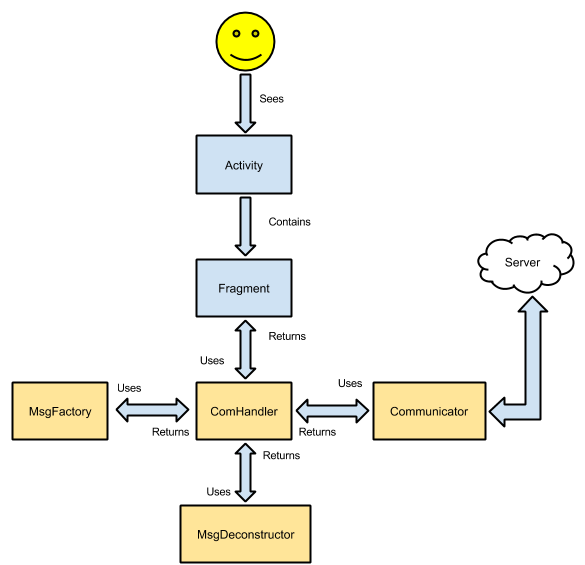
\includegraphics[width=1\textwidth]{and_system_overview.png}
		\caption{\label{fig:and_system_overview}A generalization of how the Android application works.}
	\end{figure}

	The user will interact with an activity that holds a fragment. The fragment (which contains some logic) will tell the class \verb!ComHandler! what action that should be performed. The \verb!ComHandler! will construct a message by using \verb!MsgFactory!. The message is then passed on to \verb!Communicator! which sends the message to the server with REST. The \verb!Communicator! returns the response to the \verb!ComHandler! that parses it by using the class \verb!MsgDeconstructor! and then returns it to the fragment. Hopefully, \refer{fig:and_system_overview} will bring some clarity.
	
\subsection{Package overview}
	The \verb!default! package only contains one class, \verb!SingleFragmentActivity!. This class is the base of every screen in the application. It is responsible for the navigation in the application and to inflate the correct \verb!ActionBar!. All other activities extends this 	class.

	The \verb!com! package is responsible for communication with the server. It also contains classes and methods for construction and deconstruction of JSON.

	The \verb!login! package contains the GUI and controller for the login screen. It also enables the user to select, add, edit and delete server URLs.
	
	The \verb!model! package holds information about experiments, annotations, files etc. found on the server.
	
	The \verb!processing! package is responsible for displaying processing parameters etc. for when the user wants to process a certain file.
	
	The \verb!search! package handles searches by either selecting annotations, or by manually typing in PubMed style.
	
	The \verb!search_result! package handles the results of the search by displaying the experiments found. When an experiment is selected, the files associated with the experiment is displayed.
	
	The \verb!selected_files! handles all the files that has been selected. They are sorted into raw, profile and region. The raw files can be selected for processing from here.
\pagebreak

